\section{Methods}

\subsection{Model description}

The Ecosystem Demography version 2 (ED2) model simulates plot-level vegetation dynamics and biogeochemistry~\cite{Moorcroft_2001_ED,Medvigy_2009_ED2}.
By grouping individuals of similar size, structure, and composition together into cohorts, ED2 is capable of modeling patch-level competition in a computationally efficient manner.

Relevant to this work, ED2 includes a multi-layer canopy radiative transfer model that is a generalization of the two-stream solution of Sellers (1985). \nocite{SELLERS_1985_canopy}
In its default configuration, the ED2 radiative transfer model solves for the overall hemispherical (i.e.\ diffuse) canopy albedo in two spectral ``bands''---visible and near-infrared---as a function of each cohort's leaf area index and PFT-specific parameters for leaf and wood reflectance and transmittance, canopy clumping factor, and leaf orientation factor.
The equations used are mostly adapted from the Community Land Model\cite{clm45_note}, but a summary of key features is as follows:

The direct radiation flux is modeled as an exponential attenuation curve through the canopy based on each layer's transmissivity ($\tau_r$),
which in turn is a function of the total area index ($TAI$) of the canopy layer and the inverse optical depth ($\mu_r$):

\begin{equation}\label{eq:tau_r}
  \tau_r = e ^ {- \frac{TAI}{\mu_r}}
\end{equation}

The total area index ($TAI$) is the sum of the wood area index ($WAI$) and the effective leaf area index, with the latter calculated as the product of the true leaf area index ($LAI$) and the clumping factor ($c$, defined on the interval $(0, 1)$ where 0 is a ``black hole''---all leaf mass concentrated in a single point---and 1 is a homogenous closed canopy):

\begin{equation}\label{eq:tai}
  TAI = c LAI + WAI
\end{equation}

The true leaf area index for each PFT is calcluated in two stages:
First, the total leaf biomass is calculated from the diameter at breast height via an exponential allometric equation parameterized for each PFT\@.
Second, the leaf biomass is converted to leaf area index through the PFT-specific specific leaf area (SLA).

The optical depth is calculated based on the projected area ($p$) and the solar zenith angle ($\theta$):

\begin{equation}
  \mu_r = \frac{\cos{\theta}}{p}
\end{equation}

The projected area ($p$) is a function of the leaf orientation factor ($f$):

\begin{equation}\label{eq:phi1}
  \phi_1 = 0.5 - f (0.633 + 0.33 f) \\
\end{equation}

\begin{equation}\label{eq:phi2}
  \phi_2 = 0.877 (1 - 2 \phi_1) \\
\end{equation}

\begin{equation}
  p = \phi_1 + \phi_2 \cos{\theta} 
\end{equation}

The diffuse radiation flux is more complicated because light is scattered internally within canopy layers.
Unlike the Community Land Model, which solves only for sunlit and shaded leaves,
EDR calculates the full canopy radiation profile by parameterizing the two-stream equations for each layer (as well as soil and atmosphere boundary conditions)
and then using a linear system solver to solve for the radiation profile.
For each layer, leaf and wood forward scattering ($\omega_+$) are just the sums of their respective reflectance ($r$) and transmittance ($t$) values:

\begin{equation}
   \omega_+ = r + t 
\end{equation}

Leaf and wood backscatter ($\omega_-$) are a function of their respective reflectance and transmittance values as well as the leaf orientation factor ($f$):

\begin{equation}\label{eq:backscatter_leaf}
   \omega_- = \frac{r + t + 0.25 (r - t) {(1 + f)} ^ 2}{2 (r + t)} 
\end{equation}

Overall scatter ($\iota$) and backscatter ($\beta$) of all elements in a canopy layer is modeled as the average of leaf and wood scatter, weighted by their respective area indices:

\begin{equation}\label{eq:wl}
  w_l = \frac{LAI}{LAI + WAI}
\end{equation}

\begin{equation}\label{eq:ww}
  w_w = \frac{WAI}{LAI + WAI}
\end{equation}

\begin{equation}\label{eq:scatter}
  \iota = w_l \omega_{+,l} + w_w \omega_{+,w}
\end{equation}

\begin{equation}\label{eq:backscatter}
  \beta = w_l \omega_{-,l} + w_w \omega_{-,w}
\end{equation}

The inverse optical depth for diffuse radiation ($\mu_f$) is calculated from the coefficients $\phi_1$ and $\phi_2$ (see equations~\ref{eq:phi1} and~\ref{eq:phi2}):

\begin{equation}
   \mu_f = \frac{1 - \phi_1 \ln{(1 + \frac{\phi_2}{\phi_1 \phi_2})}}{\phi_2} 
\end{equation}

Note that $\mu_f$ simplifies to 1 when orientation factor is 0 (random, spherical distribution of leaf angles).
Collectively, these coefficients are used to calculate the optical depth for diffuse radiation ($\tau_f$):

\begin{equation}
  \epsilon = 1 - 2\beta
\end{equation}

\begin{equation}
  \lambda = \frac{\sqrt{(1 - \epsilon\iota) (1 - \iota)}}{\mu_f}
\end{equation}

\begin{equation}
  \tau_f = e ^ {\lambda TAI}
\end{equation}

The remaining coefficients are described in the Community Land Model manual~\cite{clm45_note}.
% Should probably finish this as an appendix or something at some point.

By default, ED takes as parameters PFT-specific leaf and wood reflectance and transmittance values with one value each for the visible and near-infrared spectral regions. 
For this analysis, I first modified ED to take an arbitrary number of leaf and wood reflectance transmittance values.
From there on, I simulated leaf reflectance and transmittance using the PROSPECT 5 leaf RTM (see Chapters 2 and 3).
For soil and wood reflectance, I used means of the corresponding spectra from Asner (1998), resampled to 1 nm resolution. \nocite{asner_1998_biophysical}
The final coupled PROSPECT-ED canopy radiative transfer model (hereafter known as ``EDR'') has 10 parameters for each PFT\@:
5 parameters for PROSPECT (number of mesophyll layers, and area-based chlorophyll, carotenoid, water, and dry matter contents),
specific leaf area,
base and exponent for the leaf allometry,
and clumping and orientation factors.

\subsection{Sensitivity analysis}

To provide a basis for understanding the behavior of EDR, I performed a one-at-a-time sensitivity analysis to explore how its reflectance predictions vary with each leaf optical and canopy structural parameter.
To assess the mathematical foundation of the EDR canopy model (i.e.\ the Sellers two-stream scheme) without the confounding influence of multiple cohorts, I first performed this sensitivity analysis on a simulated plot containing only a single mature tree cohort.
For comparison, I also included simulations using the 4SAIL canopy radiative transfer model.
The 4SAIL model simulates four reflectance ``streams''---diffuse (hemispherical) and direct (directional) reflectance for both diffuse and direct incident radiation---\
but because EDR only simulates diffuse reflectance and its input is dominated by direct radiation (at least on sunny days, which are necessary for satellite and high-altitude airborne data), I used the ``directional-hemispherical'' output for all comparisons.
For its representation of leaf angle distribution, 4SAIL uses an ellipsoidal model that takes as input the mean leaf inclination angle ($\theta$), which is related to EDR's leaf orientation factor ($f$) by:

\begin{equation}\label{eq:orient_lidf}
  \cos \theta = \frac{1 + f}{2}
\end{equation}

Unlike EDR, 4SAIL does not account for canopy clumping.
(4SAIL does have a ``hot spot'' parameter to account for strong bi-directional reflectance effects from structurally heterogeneous canopies, but this parameter only affects the bi-directional reflectance, which was not used in this analysis).

To investigate the way EDR models interactions between canopy layers, I also performed a similar sensitivity analysis on a simulated plot with two cohorts---a dominant early successional cohort and a sub-dominant mid-successional cohort.
I examined the sensitivity of total canopy reflectance to the optical properties of both the dominant and sub-dominant cohort, and looked at how this sensitivity was affected by clumping in the upper cohort.

\subsection{Model calibration}

For model calibration, I selected 47 sites from the NASA Forest Functional Types (FFT) field campaign that contained plot-level inventory data (stem density, species identity, and DBH) coincident with observations of the NASA Airborne Visible/Infrared Imaging Spectrometer (AVIRIS).
These sites are mostly located in the United States Upper Midwest with several sites also in upstate New York and western Maryland, and include stands dominated by either evergreen or deciduous trees and spanning a wide range of structures, from dense groups of saplings (bottom right) to sparse groups of large trees (top left) (Figure~\ref{fig:sites}).
Based on ED's PFT definitions, these sites contained a total of five different temperate plant functional types: Early successional hardwood, northern mid-successional hardwood, late successional hardwood, northern pine, and late successional conifer.

\begin{figure}
  \centering
  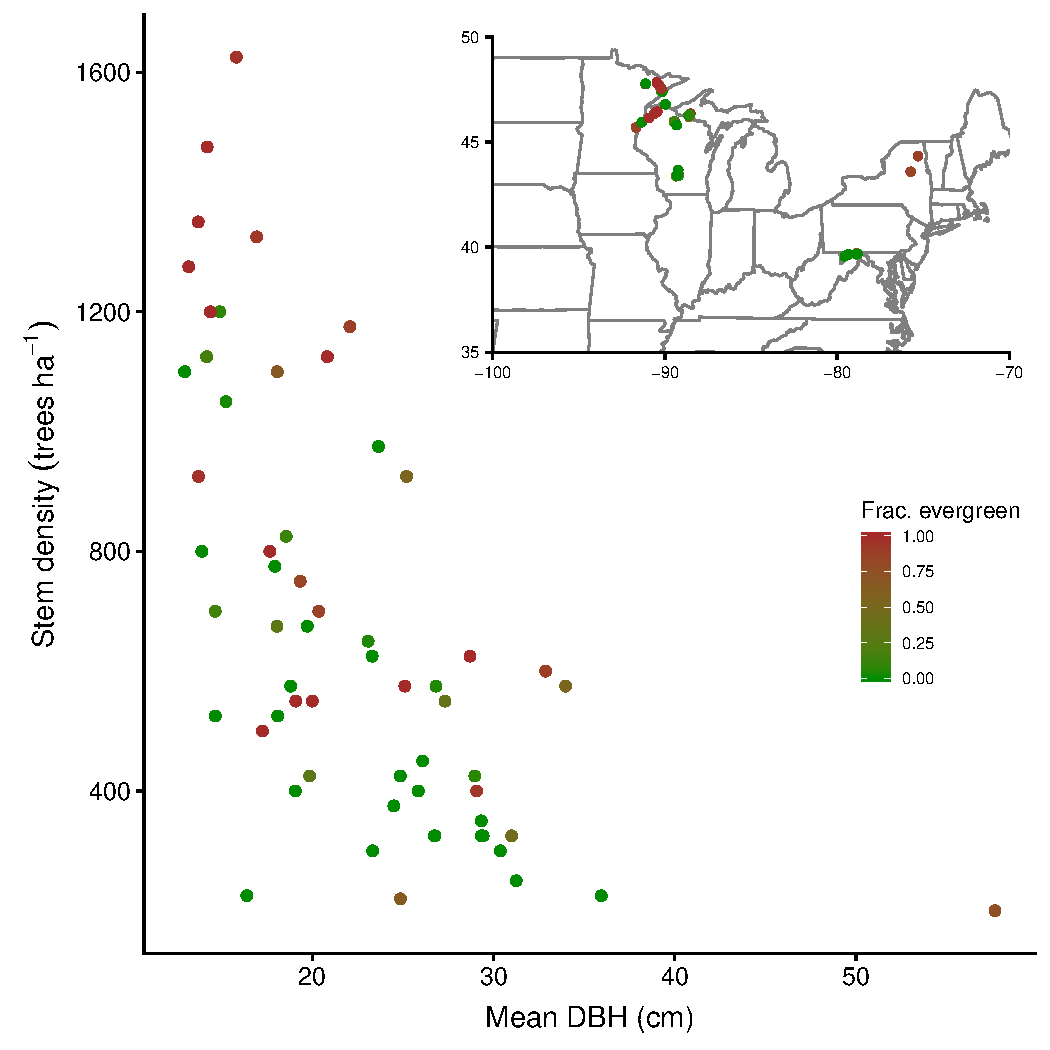
\includegraphics[width=\textwidth]{figures/sites_both.pdf}
  \caption{\
    Sites selected for analysis, in ``stand structure'' (\textit{main figure}) and geographic (\textit{inset}) space.
    Colors indicate the fraction of the stand that is made up of evergreen PFTs.
    Large points with labels indicate sites that were selected for forward simulations.
  }\label{fig:sites}
\end{figure}
% * <fer.istem@gmail.com> 2018-05-02T19:51:35.047Z:
% 
% not sure if it matters but the deciduousness gradient is not detectible from the color scheme, all points seem either 0 or 1 to me
% 
% ^.
% TODO: Change colors to be top cohort
% TODO: Remove the site labels

I calibrated EDR using the same general Bayesian inversion as in Chapter 3.
The inversion fit all sites simultaneously, such that at every MCMC iteration, the algorithm proposed a set of all parameter values for each PFT and simulated spectra for each site based on its observed composition and structure.
Because of unrealistic values in the shortwave infrared spectral region in the AVIRIS observations, likely caused by faulty atmospheric correction, I only calibrated the model with observations from 400 to 1300 nm.
In addition, I changed the fixed variance model used in Chapters 2 and 3 to a two-parameter heteroskedastic variance model ($\sigma = a + bX$) to account for the fact that both model and observation errors are typically proportional to reflectance values.
To generate the initial history state files required by EDR, I ran ED2 itself for one day in midsummer (July 1), starting from vegetation initial conditions based on observed composition and structure.

For priors on the five PROSPECT parameters and specific leaf area, I performed a hierarchical multivariate analysis (see Chapter 1) on PROSPECT parameters estimated from chapter 3 and, where available, direct measurements of specific leaf area. 
For priors on the leaf biomass allometry parameters, I fit a multivariate normal distribution to allometry coefficients from Jenkins et al.~(2003, 2004) using the \texttt{PEcAn.allometry} package. \nocite{jenkins_2003_allom,jenkins_2004_allom} 
For the clumping factor, I used a uniform prior across its full range (0 to 1), and for the leaf orientation factor, I used a weakly informative re-scaled beta distribution centered on 0.5.

To alleviate issues with strong collinearity between the two allometry coefficients and the specific leaf area, I decided to remove the allometry exponent coefficient (but not the intercept) from the calibration by fixing it at its prior mean for each plant functional type.
Doing so dramatically improved the stability of the inversion algorithm and the accuracy of the results.

I evaluated the performance of the calibrated model by comparing the posterior credible intervals of modeled spectra against the AVIRIS observations at each site.
To assess the role of model structure in predictive error, I also included predictions using the 4SAIL model parameterized with the posterior means from the EDR calibration (except for clumping factor, which is absent from 4SAIL).
In addition, I compared model predictions of leaf area index (which depend on parameters calibrated in the model) against field observations.
